
%! FerriganHash.tex
%! Author = Vincent Ferrigan <ferrigan@kth.se>
%! Date = 2022-10-20


% Preamble
\documentclass[a4paper, 11pt]{article}
% Packages
\usepackage[T1]{fontenc}
% \usepackage[utf8]{inputenc} % ska den tas bort iom lua?
% \usepackage[utf8]{luainputenc}
\usepackage[english]{babel}
\usepackage{fontspec}
\usepackage{microtype}
\setmonofont{DejaVu Sans Mono}[Scale=MatchLowercase]
\usepackage{listings}
\usepackage{minted}
\usepackage{latexsym,exscale,stmaryrd,amsmath,amssymb}
\newtheorem{definition}{Definition}
\usepackage{unicode-math}
\usepackage{lmodern}
\usepackage{enumitem}
\usepackage{subcaption}
\usepackage{graphicx}
\usepackage{hyperref}
\usepackage{multirow}
\usepackage{diagbox} % For diagonal lines in tabular
\usepackage{booktabs}
% \usepackage{paralist}

%% Om jag vill referera till ett kod verb av något slag, som void null Int etc
% \usepackage{tcolorbox}
% \newtcbox{\somestuffstyle}{on line,boxrule=0pt,boxsep=0pt,colback=lightgray,top=1pt,bottom=1pt,left=1pt,right=1pt,arc=0pt,fontupper=\ttfamily}

\usepackage[
    backend=biber,
    % hyperref=true,
    maxnames=3, 
    minnames=1, 
    nohashothers=false
    bibencoding=utf8, % eventuellt
    style=apa,
    % citestyle=apa,
    pluralothers=true,
    natbib=true
    % sorting=nyt
    % autocite=inline
    ]{biblatex}
\DefineBibliographyStrings{english}{andothers={et. al}, and={&}}
\DeclareLanguageMapping{english}{english-apa}
\addbibresource{references.bib} % hör till referenser
% \addbibresource{../references.bib} % hör till referenser
% \usepackage[backend=biber,style=apa,natbib=true,sorting=nyt]{biblatex}
% \addbibresource{references.bib}
% \usepackage{natbib}
\usepackage{csquotes}
\usepackage[nottoc]{tocbibind}
\usepackage{xcolor}
\usepackage{siunitx}
\usepackage{tikz}
\usepackage[font=small,labelfont=bf]{caption}
% Addiding JuliaMono
\newfontfamily \JuliaMono {JuliaMono-Regular.ttf}[
    Path      = ./,
    Extension = .ttf
    ]
\newfontface \JuliaMonoMedium{JuliaMono-Regular}
\setmonofont{JuliaMonoMedium}[
    Contextuals=Alternate
]
\usetikzlibrary{matrix, positioning}
\tikzset{
node of list/.style = { 
             draw, 
             fill=gray!20, 
             minimum height=6mm, 
             minimum width=6mm,
             node distance=6mm
   },
link/.style = {
     -stealth,
     shorten >=1pt
     },
array element/.style = {
    draw, fill=white, 
    minimum width = 6mm,
    minimum height = 10mm,
}
}

% \def\LinkedList#1{%
%   \foreach \element in \list {
%      \node[node of list, right = of aux, name=ele] {\element};
%      \draw[link] (aux) -- (ele);
%      \coordinate (aux) at (ele.east);
%   } 
% }
\def\LinkedList#1{%
  \foreach \element in \list {
     \node[node of list, right = of aux, name=ele] {\element};
     \node[node of list, name=aux2, anchor=west] at ([xshift=-.4pt] ele.east) {};
     \draw[link] (aux) -- (ele);
     \coordinate (aux) at (aux2);
   }
   \fill (aux) circle(2pt);
}

\title{Hash tables\\ \small{ID1021 Algorithms and Data structures}} %%TODO VILKEN RUBRICERING
\author{Vincent Ferrigan}

\date{\today}

\begin{document}
    \maketitle
    \section*{Introduction}
    \label{sec:introduction}
    In this study, the performance and mechanism of \emph{Hash Tables}, a 
    data structure supporting \emph{Symbol Tables}, 
    also known as \emph{Dictionaries}, was studied and analyzed.
    Besides comparing the different ways of storing data in Hash Tables,
    the dictionary operations \emph{insertion} and \emph{search} were also compared
    with storing data in the more basic data structure, like \emph{linked lists} and \emph{arrays}, 
    with their equivalent algorithms \emph{Linear Search}, \emph{Binary Search} and 
    \emph{Direct Addressing}. 
    (The latter being more of a ''simple technique'' of storing or
    ''addressing data'' in memory rather than an algorithm.) 
    
    The above-mentioned comparisons were done through different types of benchmarking. 
    The authors intent is to reach certain conclusions regarding 
    the balance between the time and space complexity of hash tables. 

    \section*{Methods}
    \label{sec:methods}
    All the Data Structures and Algorithms were implemented in \emph{Julia}.
    The Code was mostly written in \emph{VSCode} and run on \emph{Julia 1.8.0}.
    Quick-fixes and editing was, however, done in \emph{Vim}. 
    Some scripts were executed from the \emph{REPL terminal},  while others (e.g.
    when using data frames, performing benchmarks and producing plots) 
    were executed from the \emph{Jupyter Notebook}. 
    % Ska jag lägga till länk till min github? To follow the progress.....
    % men då måste notebooken läggas upp.
    
    \subsection*{Tools and packages}
    All tests were performed with the built-in package \emph{Test} and 
    iterative development was made possible through 
    \emph{Revise.jl} -- the latter operates by continuously
    scanning the source code for changes, even changes in functions defined in
    other modules (including modules written in different files). 
    Version control was done through \emph{Git} and \emph{Git-Hub} and the paper
    was written in \emph{\LaTeX} and compiled with \emph{LuaTeX} and \emph{Biber}.
    
    The benchmark data was constructed, manipulated and visualized through
    \emph{DataFrames.jl} and \emph{Plots.jl}, 
    while readable formatting was produced through 
    \emph{Formatting.jl} and \emph{Unitful.jl}. 

    \subsection*{The JIT}
    Julia has a just-in-time (JIT) compilation -- which means that the code is
    dynamically compiled during program run time.     
    It takes time for the JIT compiler to 
    initially load the code and compile it. Therefore, in order not to skew the
    results, \emph{warm-up calls} were performed on certain parts of the code
    before they were benchmarked. This to avoid including 
    compilation time. The warm-up calls were done with the @timed macro prior to
    benchmarking.

    \section*{The Data Structure and their operations} %% TODO CHANGE DEPENDING ON ASSIGNMENT
    This section briefly describes Hash Tables - a data structure that supports
    \emph{Symbol Tables} -- also known as \emph{Dictionaries}. 
    For clarity, the reader will be given an account of the mechanism 
    behind storing data, \emph{values}, in a table 
    that later can be looked up with a \emph{key}. 
    The subsections will go through the key differences between 
    \emph{Direct-}, \emph{Open-} and \emph{Closed Addressing} and their
    \emph{collision resolution} techniques when mapping keys to values; 
    \emph{Chaining} with singly linked lists
    and \emph{Linear Probing}. 
    
    The reader will also be provided with code examples when necessary.
    
    \subsection*{1-based indexing and other Conventions}
    It is important for the reader to note that Julia uses a \emph{one-based-numbering
    convention}, (i.e. array indices start from 1 to N) and that one dimensional
    arrays are called vectors.  
    For consistency, the author has chosen to refer to one dimensional
    arrays as vectors and apply the 1-based convention when numbering
    sequences of elements more broadly. \emph{Modular hashing} 
    will therefore differ -- 
    returning a value in the range $(0,y]$ rather than $[0,y)$. E.g.
    \mintinline{julia}{mod1(11, 11)} returns $11$ and not $0$. This also
    applies when wrapping around vector indices during \emph{linear probing}
    and \emph{hash table resizing}.
        
    Unlike other languages, Julia objects cannot be ''null'' by default. The
    equivalent of \lstinline[language=Python]{None} in Python or
    \lstinline[language=C]{NULL} and \lstinline[language=C]{void} in C is
    \mintinline{julia}{Nothing}. The Julia convention is to return the value
    \mintinline{julia}{nothing}, which is a singleton instance of type
    \mintinline{julia}{Nothing}, when such a side effect is
    desired. 
    
    Function names that end with a bang (!) mutates the arguments it receives. 
    This name suffix is by convention in Julia. 
    \subsection*{Addressing Tables}

    xxxxxx
    Closed addressing requires ... hashing, 
    what hashing did we choose and other exists and why.

    Load factor, that c.a. requires linked lists, 

    Open Addressing
    - Load factor, that it requires resizing and rehashing
    ... ref to discussion. 
    xxxxx

    \begin{figure}[h]
    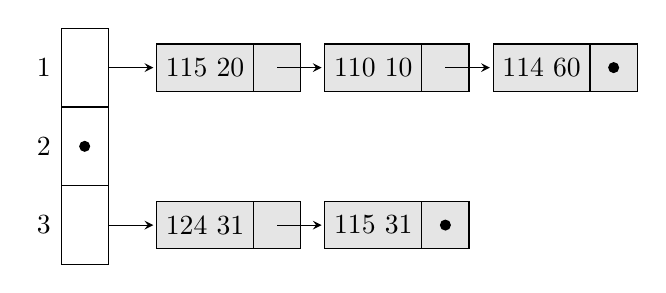
\begin{tikzpicture}
\foreach \index/\list in {1/{115 20, 110 10, 114 60}, 2/{}, 3/{124 31, 115 31}}  
{

   \node[array element] (aux) at (0,-\index) [label=left:\index]{};
   \LinkedList{\list}
}
\end{tikzpicture}
    \caption{Closed Addressing.
Collision resolution by chaining. Each slot of the vector contains a reference
to a singly-linked list containing
key-value pairs with the same hash value.}
    \label{code:ClosedAddressing}
    \end{figure}

    \begin{figure}[h]
        \centering
        %% you can have several subfigures or minteds
        %% TODO: add label/caption on minted, e.g. Outer Method
    \begin{minted}[
        label= XXXXXXX, 
        linenos, 
        % breaklines, 
        frame = single, 
        fontsize=\footnotesize]{julia}

    \end{minted}
    \caption{xxx} %% TODO ADD CAPTION
    \label{code:xxx} %% TODO ADD LABEL
    \end{figure}

    \clearpage
    \section*{Results}
    \label{sec:results}
    \subsection*{The lookup benchmark}
    xxxxxx describe benchmark, ref to \autoref{tab:lookup}


    \begin{table}[h]
        \centering
        \small
\begin{tabular}{lrrrr} % TODO: correct columns
    \toprule
    & \multicolumn{4}{c}{\textbf{Key}} \\\cmidrule(lr){2-5}
    \textbf{Algorithm} & \multicolumn{1}{c}{"115 15"} &\multicolumn{1}{c}{"994 99"}& \multicolumn{1}{c}{$11515$}&\multicolumn{1}{c}{$99499$}\\
    \cmidrule(lr){1-1}
    \cmidrule(lr){2-5}
    Linear Search      &\SI{14}{\nano\second}   &\SI{32871}{\nano\second}   &\SI{17}{\nano\second}  &\SI{7432}{\nano\second}\\
    Binary Search      &\SI{107}{\nano\second}  &\SI{132}{\nano\second}     &\SI{119}{\nano\second} &\SI{134}{\nano\second} \\
    Direct Addressing  & \multicolumn{2}{c}{n/a}                       &\SI{15}{\nano\second}  &\SI{15}{\nano\second}  \\
    \bottomrule
\end{tabular}
    \caption{xxxx} % TODO: add caption
    \label{tab:lookup} % TODO: add correct label
    \end{table}
\hline

    % \begin{figure}[h] % You can have subfigures !! If necessary 
    %     \centering
    %     \includegraphics[width=0.8\textwidth]{./input/xxxxx.pdf} %% TODO: add pdf
    %     \caption{xxxx}%% TODO: add caption
    %     \label{fig:fig1} %% TODO: add correct fignbr /label
    % \end{figure}
    \subsection*{Collisions}

    \subsection*{Attempts}

    \section*{Discussion}
    \label{sec:discussion}
    xxxxxx
    \section*{EXAMPLE SECTION WITH REF}
    xxxxxx 
    \hyperref[sec:results]{Results}
    xxxxxx 
    \autoref{code:xxx}
    % xxxxxx 
    % \autoref{fig:fig1}

    xxxxxx with with apren cite 
    \parencite{Segeqick2011Alg4th}

    xxxxxx with with paren cite 
    \parencite{CormenThomasH2022ItA}

    xxxxxx with with text cite 
    \textcite{Segeqick2011Alg4th}
    xxx

    xxxxxx with with text cite 
    \citep{Segeqick2011Alg4th}
    xxx

    xxxxxx with with text cite 
    \citet{Segeqick2011Alg4th}
    xxx

    xxxxxx with with text cite 
    \citep{CormenThomasH2022ItA}
    xxx


    %\section{Appendix A - Referenser}
\printbibliography
\end{document}